\chapter{計算結果}
VASPを導入したMoment法,Lennerd-Jones型経験的ペアポテンシャルを用いた従来のMoment法,MedeA, Phonopyによる結果の比較を行う.図内のラベルには結果をそれぞれ,MomentVASP, MomentLJ, MedeA, Phonopyと表記しており,今後はこの名称で扱うことにする.
\section{熱膨張}
熱膨張による最近接原子間距離の温度依存を図\ref{fig:heatexpantion}に示す.この結果から得られる線膨張係数を図\ref{fig:heatexpantion2}に実験値とともに示す.
MomentLJの0Kの最近節原子間距離が他の結果と大きな差があるのは使用したペアポテンシャルの最安定距離がVASPによる基底状態の最安定距離とずれているためである.また,高温域で現実的ではない加速的な熱膨張をしており$k$,$\gamma$が負の値を取り計算不可となり結果が途切れている.MomentLJとMomentVASPを比較すると,後者がMedeA, Phonopy, 実験値に近い結果を出していることがわかる.
MomentLJ,MomentVASPともに100K以下の低温域で現実的ではない熱膨張を示しており\ref{sec:he_100k}節で原因の検証を行う.
MomentVASPのCu, Ag, Auに着目するとAgの高温域での加速的な熱膨張を除いてPhonopy, MedeAに劣らず実験値に近い結果が出ている.
Phonopy, MedeAのAuの結果が大きく熱膨張しているのは,格子を大きく伸ばしたAuにおいてPhonon状態密度に負の値が多く混ざり自由エネルギーが正確に算出できなかったためである.
そのため,AuはPhonon-DOS法では熱膨張を上手く再現できなかったが,Phononとは違うアプローチで計算を行うMomentVASPでは実験値に近い熱膨張係数を得ることができている.
Alに関してはMedeA, Phonopyが上手く実験値を再現できているがMomentVASPでは熱膨張が小さいという結果となった.
これらの結果と図\ref{fig:allkgamma}を比べると$k$, $\gamma$の傾きが変わらなければ直線的な熱膨張になることがわかる.
MomentVASPのAgの高温域における熱膨張は$\gamma$の傾きの変化が他の元素に比べて大きいことが原因だと考えられる.
\begin{figure}[htbp]
 \begin{minipage}[b]{0.5\linewidth}
  \centering
  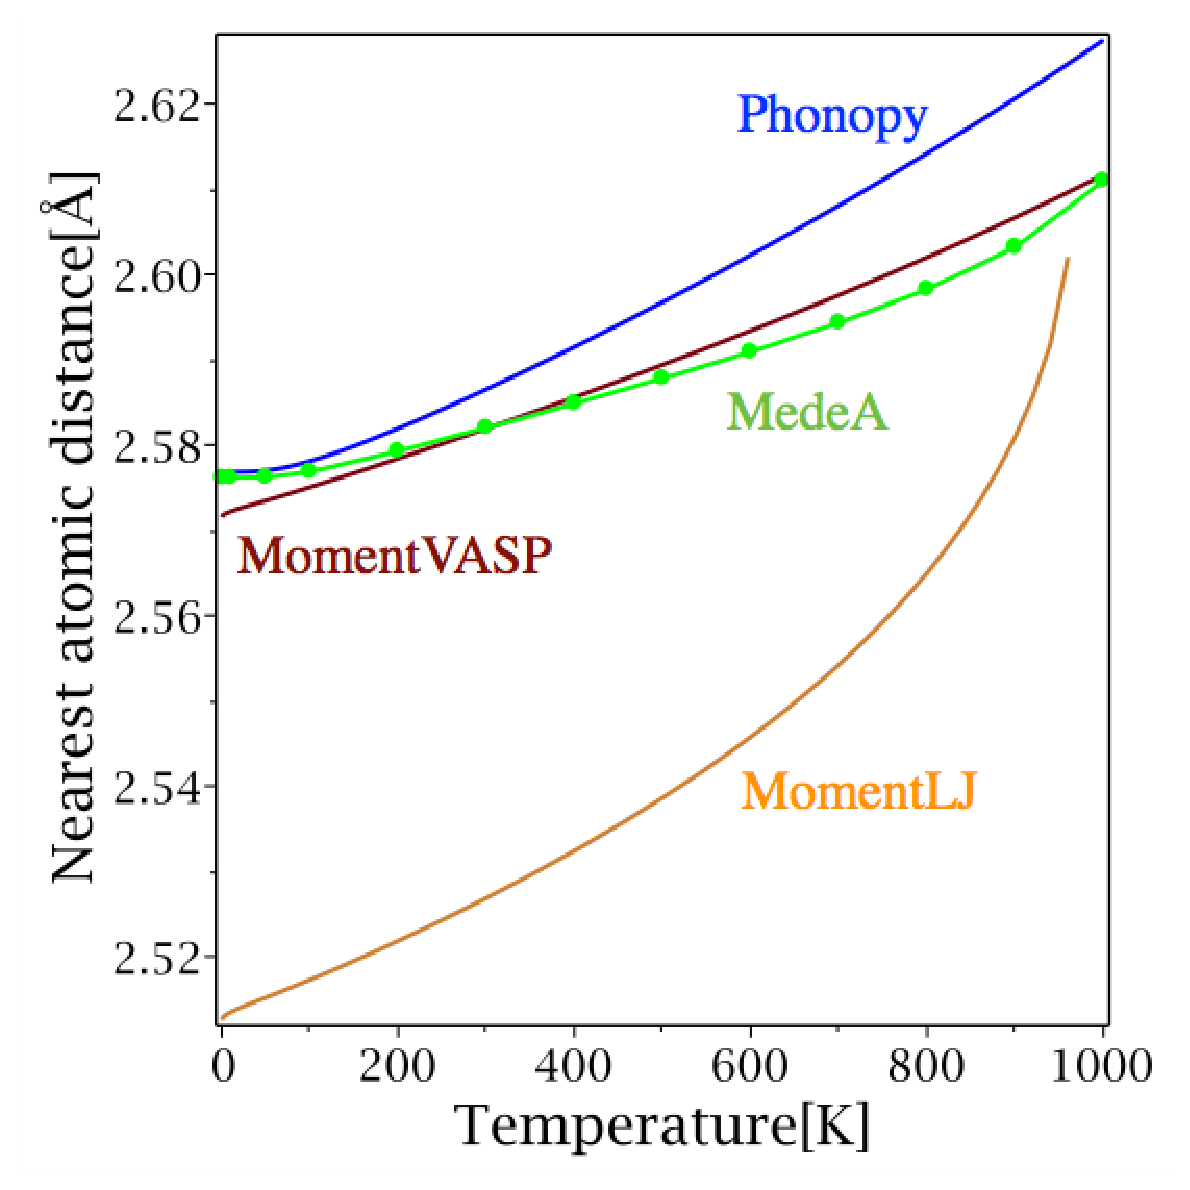
\includegraphics[keepaspectratio, scale=0.42]
  {../image_result/Cu_lat_label.eps}
  \subcaption{Cu.}\label{he1}
 \end{minipage}
 \begin{minipage}[b]{0.5\linewidth}
  \centering
  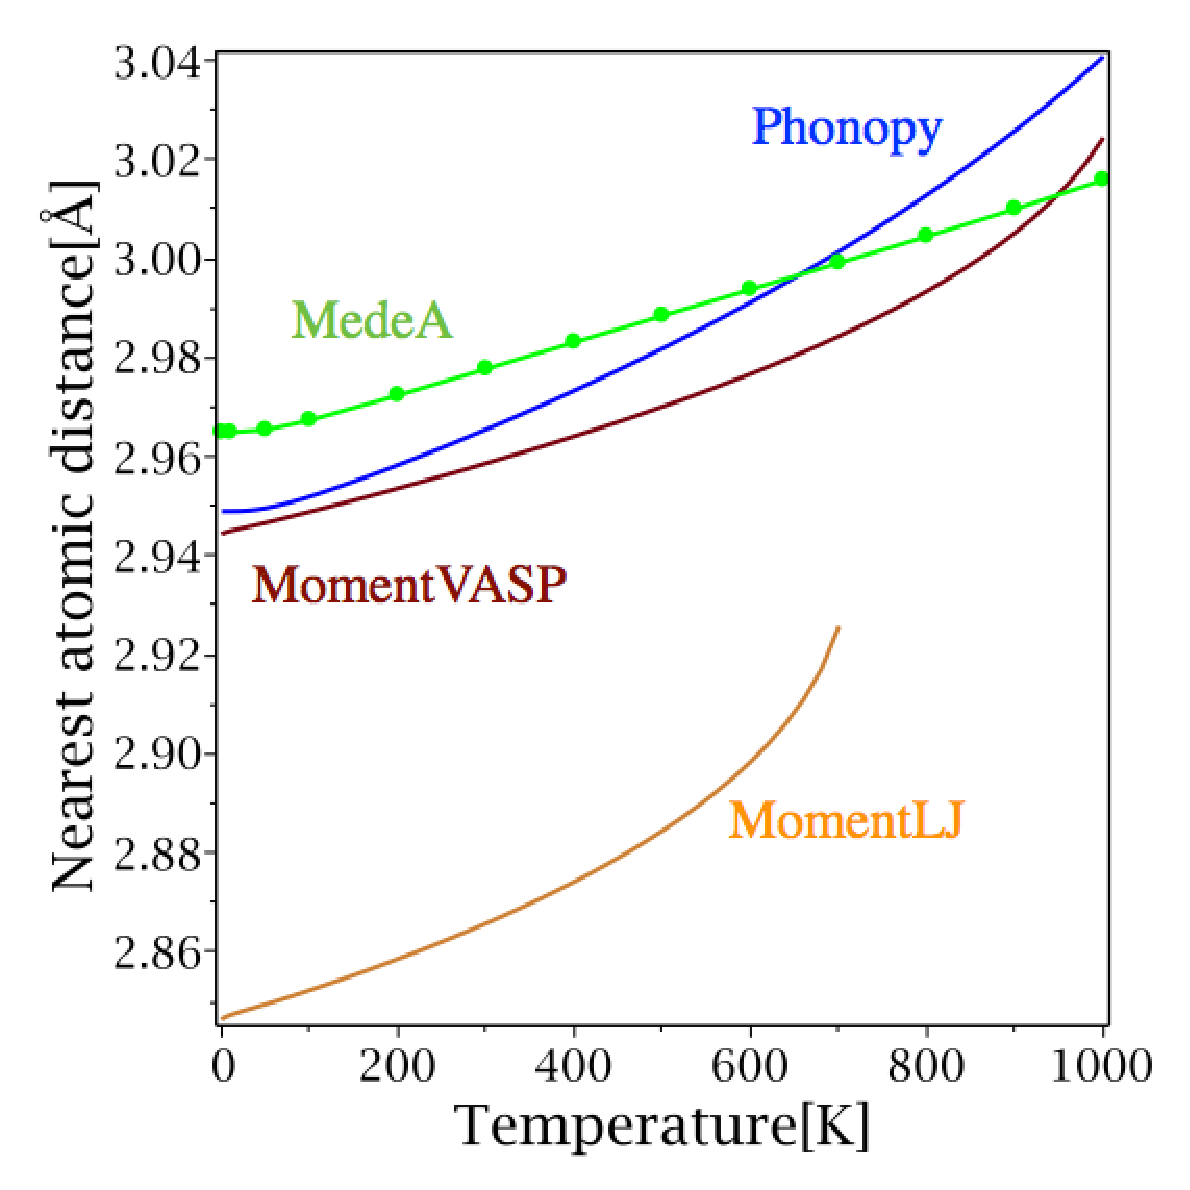
\includegraphics[keepaspectratio, scale=0.42]
  {../image_result/Ag_lat_label.eps}
  \subcaption{Ag.}\label{he2}
 \end{minipage}
 \hspace{10cm}
 \begin{minipage}[b]{0.5\linewidth}
  \centering
  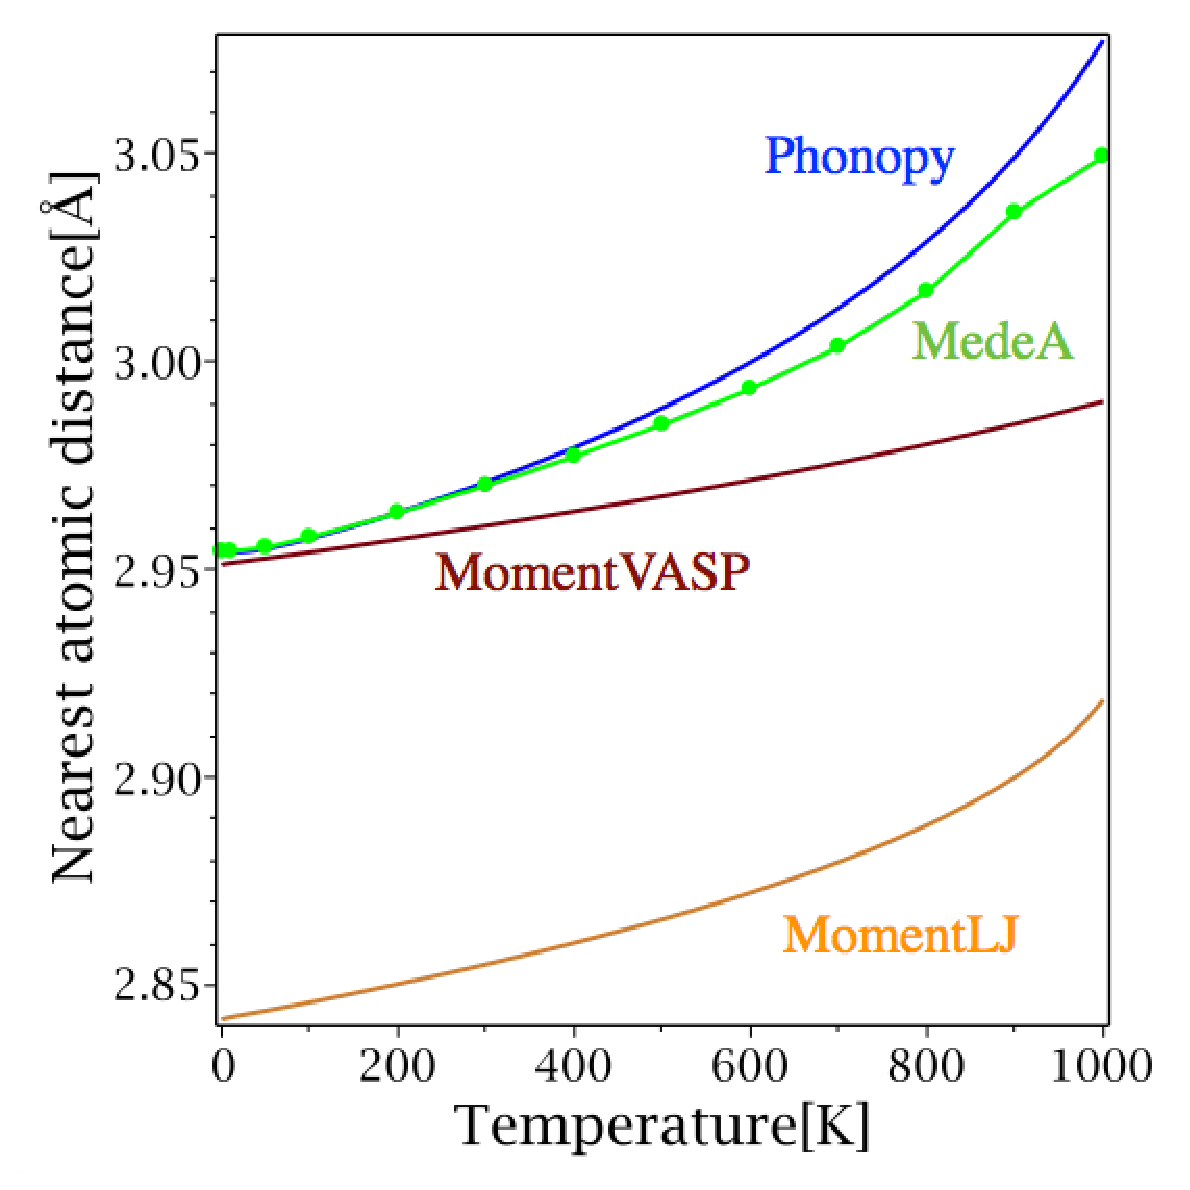
\includegraphics[keepaspectratio, scale=0.42]
  {../image_result/Au_lat_label.eps}
  \subcaption{Au.}\label{he3}
 \end{minipage}
 \begin{minipage}[b]{0.5\linewidth}
  \centering
  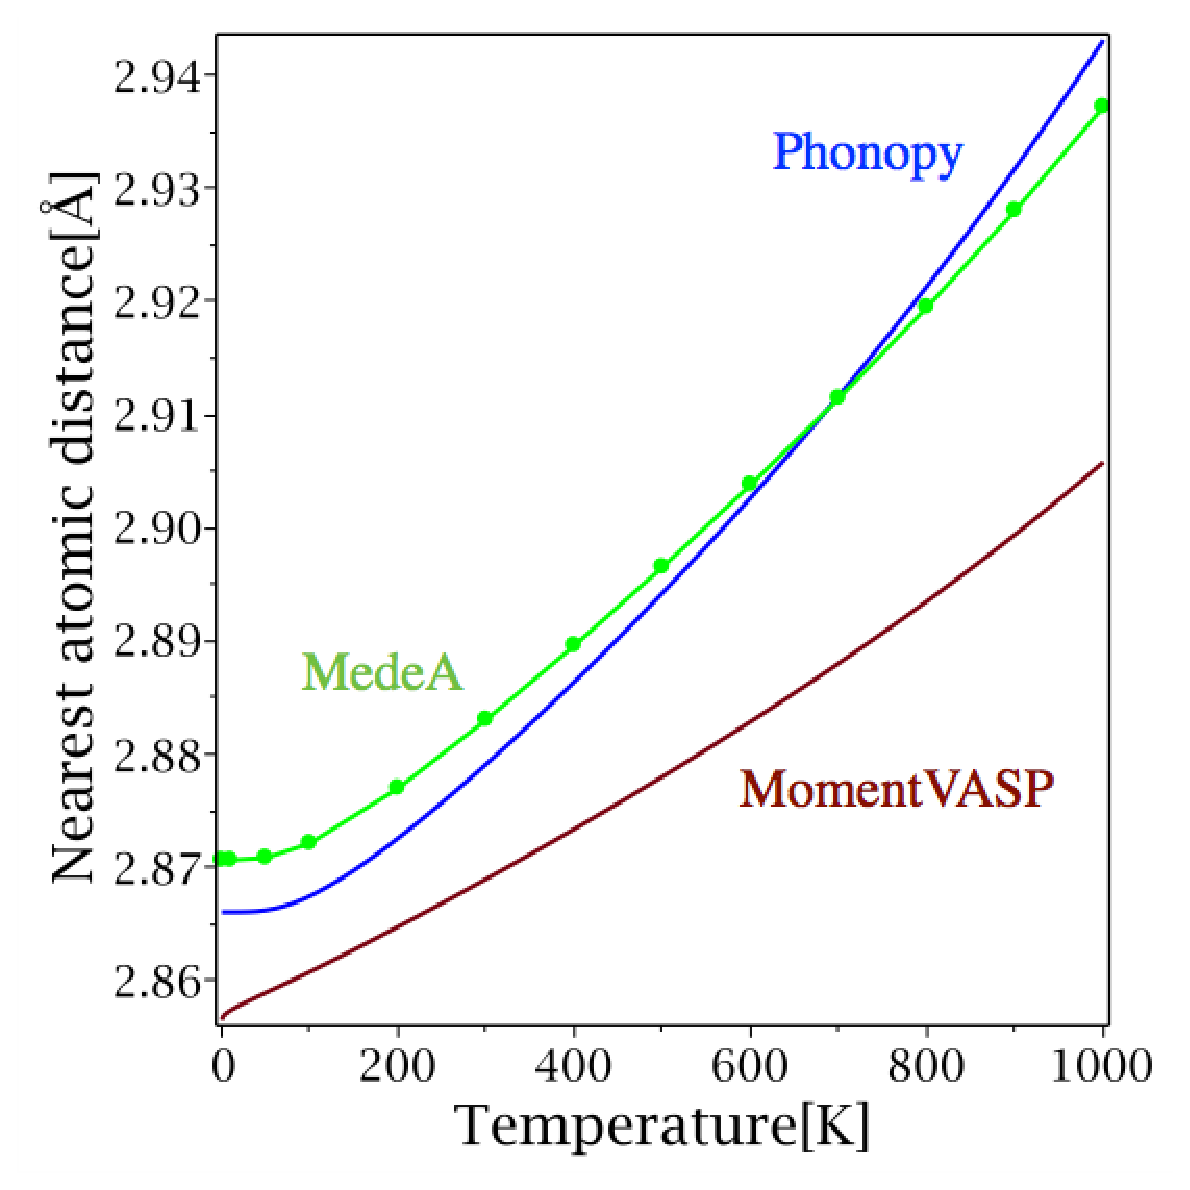
\includegraphics[keepaspectratio, scale=0.42]
  {../image_result/Al_lat_label.eps}
  \subcaption{Al.}\label{he4}
 \end{minipage}
 \caption{最近接原子間距離の温度依存性.}\label{fig:heatexpantion}
\end{figure}

\begin{figure}[htbp]
 \begin{minipage}[b]{0.5\linewidth}
  \centering
  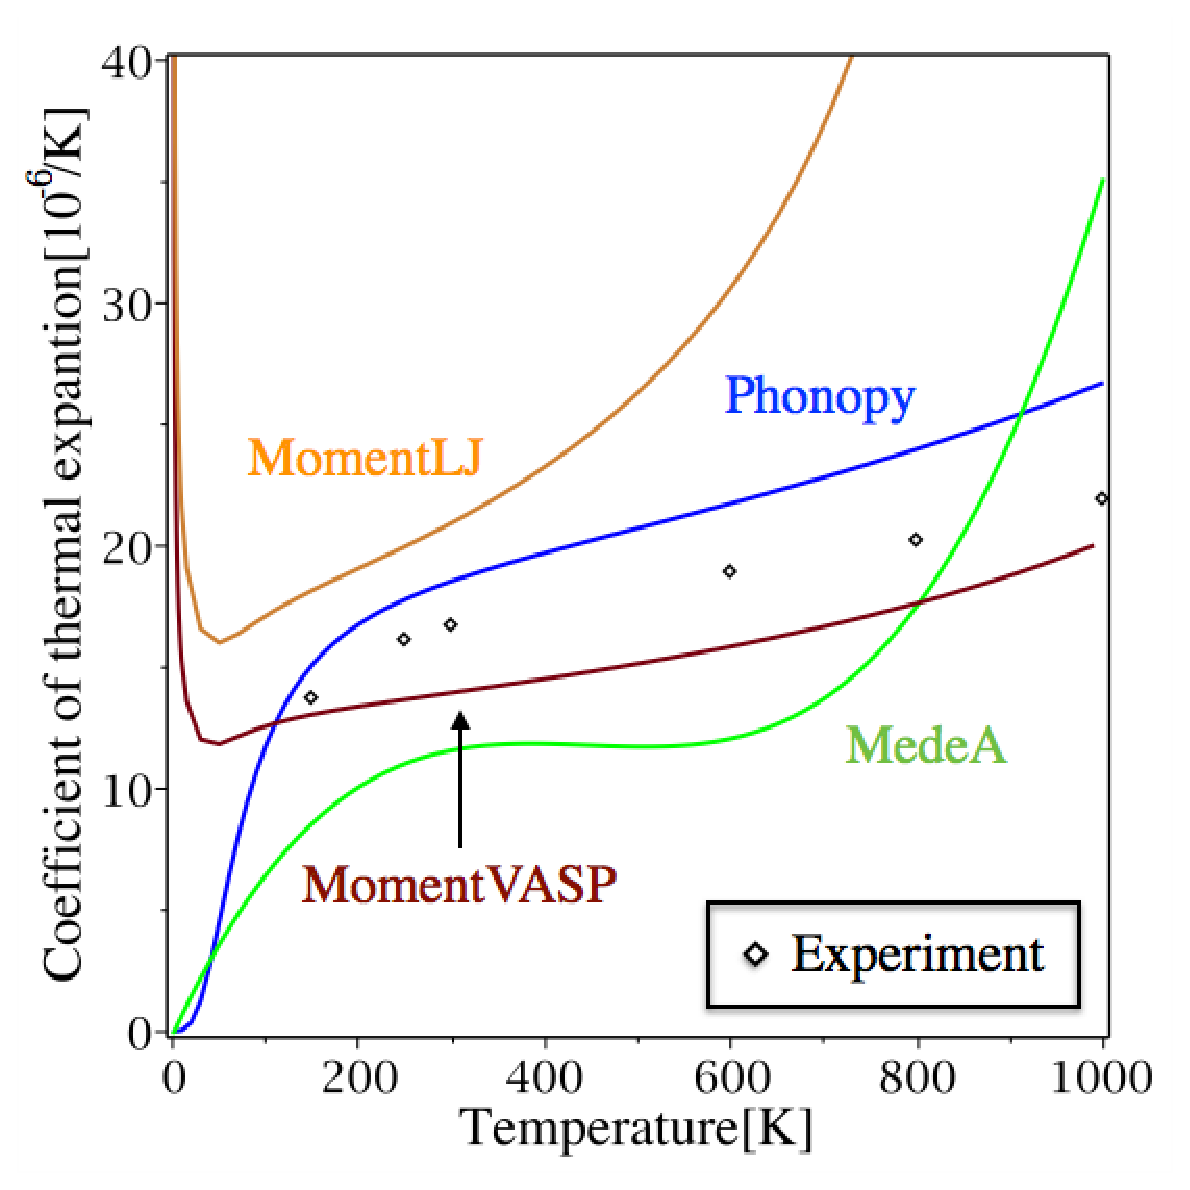
\includegraphics[keepaspectratio, scale=0.42]
  {../image_result/Cu_TEcoeff_label.eps}
  \subcaption{Cu.}\label{he5}
 \end{minipage}
 \begin{minipage}[b]{0.5\linewidth}
  \centering
  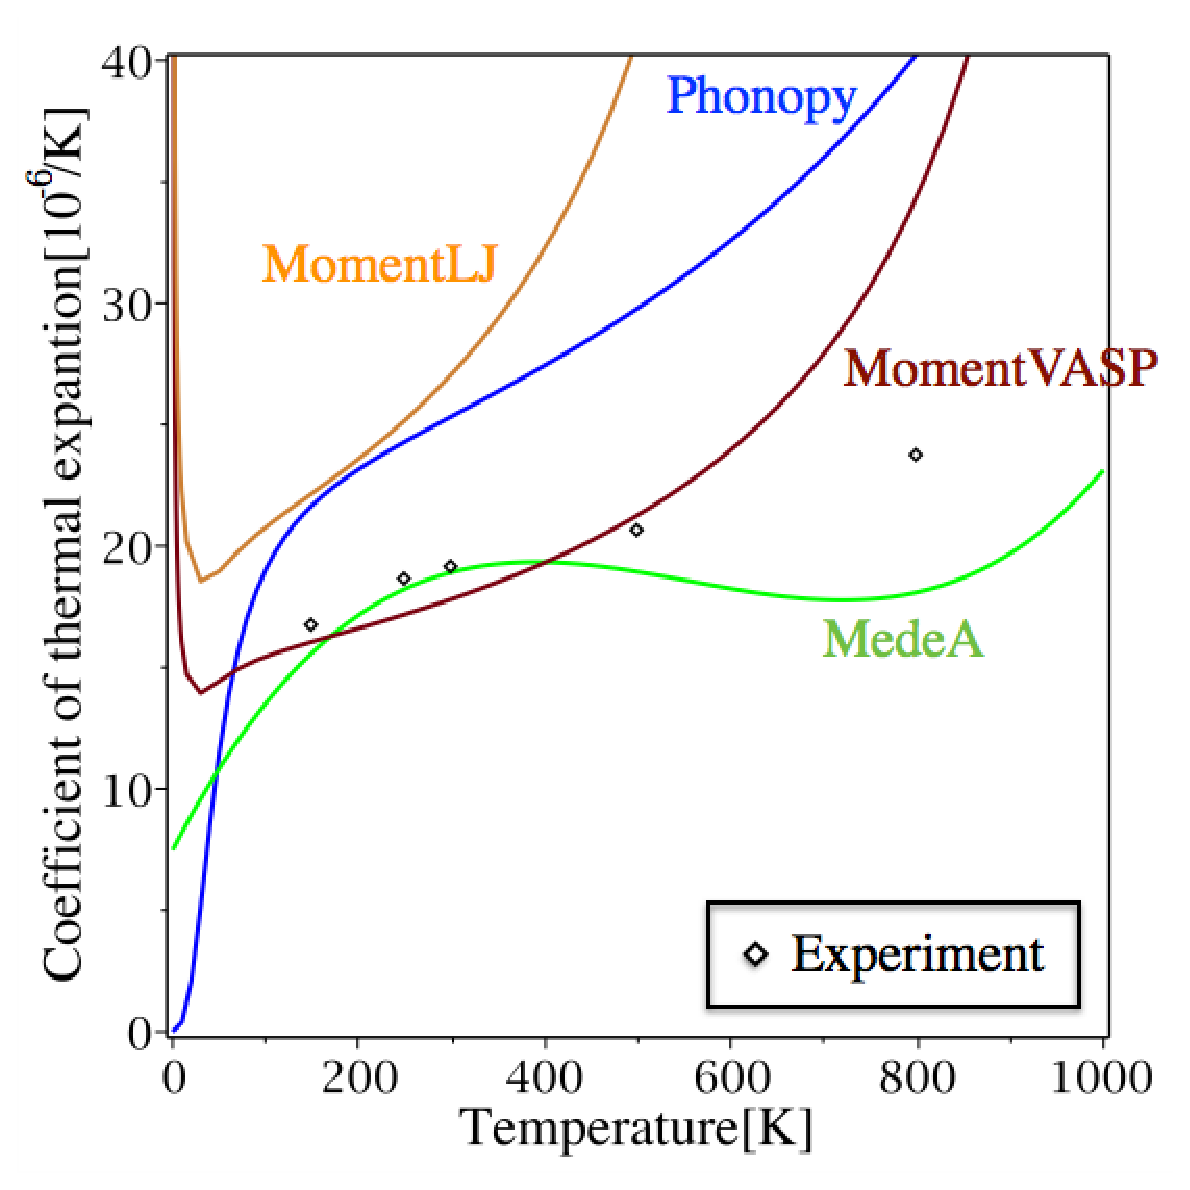
\includegraphics[keepaspectratio, scale=0.42]
  {../image_result/Ag_TEcoeff_label.eps}
  \subcaption{Ag.}\label{he6}
 \end{minipage}
 \hspace{10cm}
 \begin{minipage}[b]{0.5\linewidth}
  \centering
  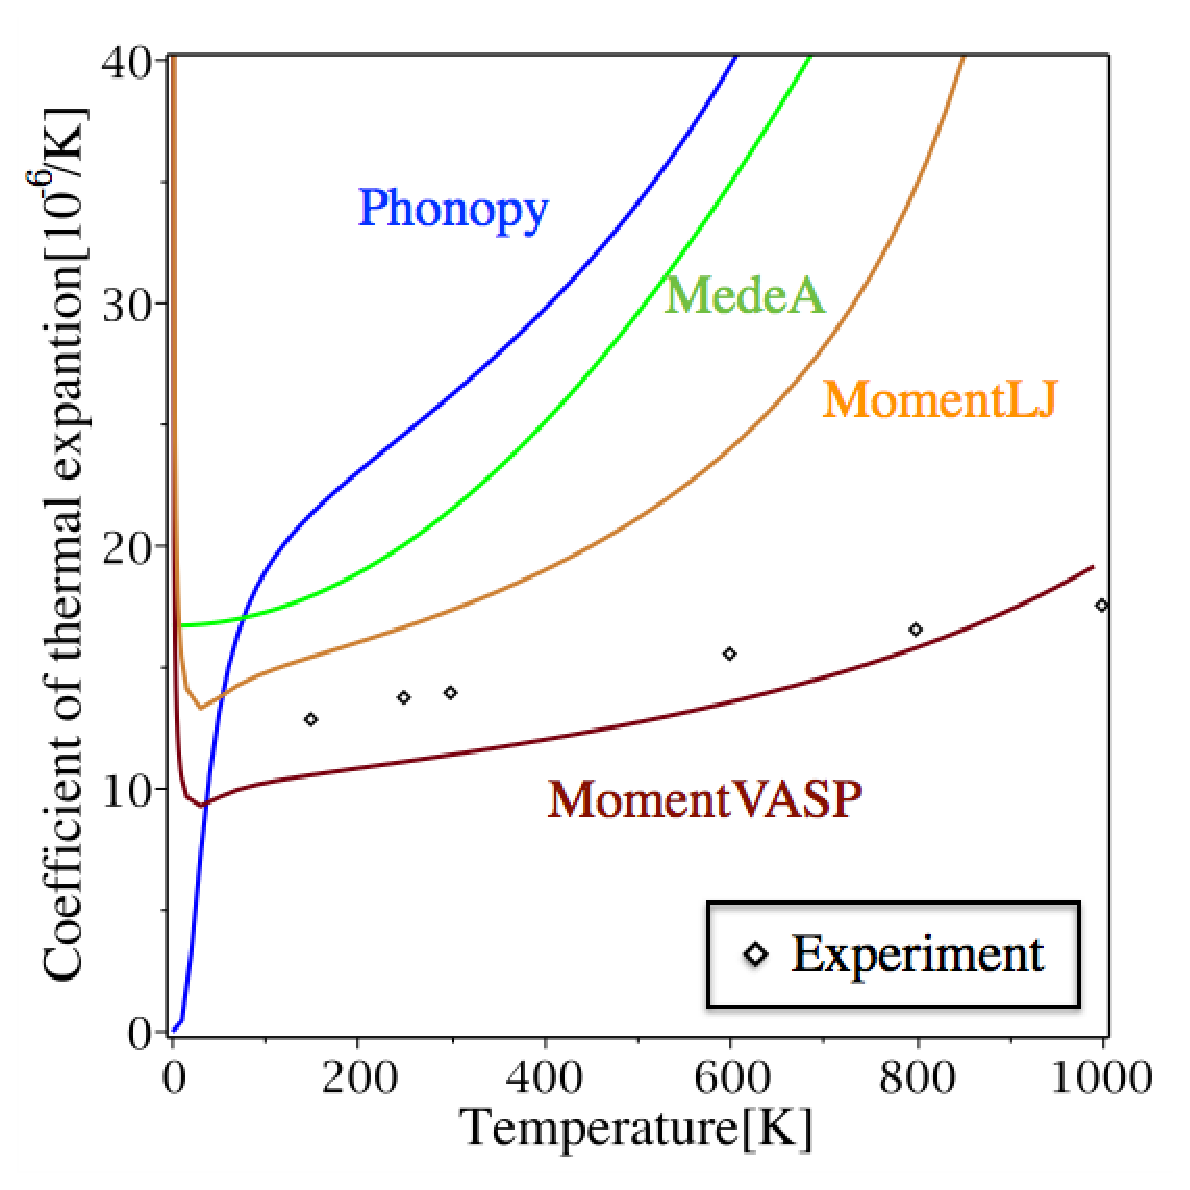
\includegraphics[keepaspectratio, scale=0.42]
  {../image_result/Au_TEcoeff_label.eps}
  \subcaption{Au.}\label{he7}
 \end{minipage}
 \begin{minipage}[b]{0.5\linewidth}
  \centering
  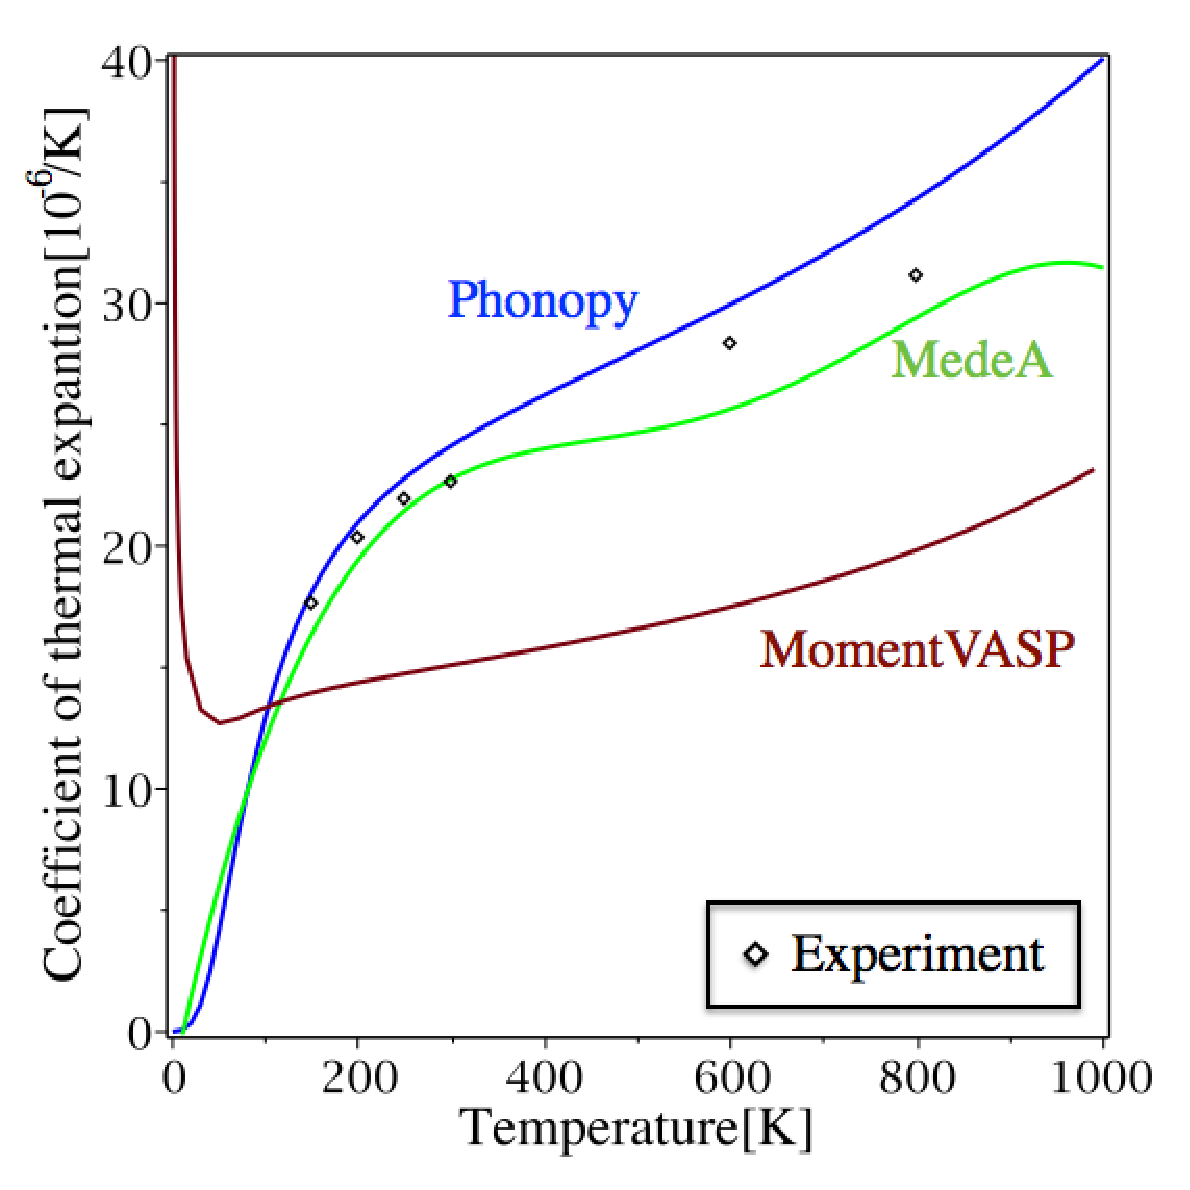
\includegraphics[keepaspectratio, scale=0.42]
  {../image_result/Al_TEcoeff_label.eps}
  \subcaption{Al.}\label{he8}
 \end{minipage}
 \caption{線膨張係数の温度依存性.}\label{fig:heatexpantion2}
\end{figure}

\section{内部エネルギー$U_0$を含まない自由エネルギー}
Medea, Phonopyの熱膨張の結果に不安があるため,まずはVASPによる構造最適化によって得られる格子定数のもとで一般的な体積一定の熱膨張を考慮していない自由エネルギーとの比較を行う.
MedeA, Phonopyによる自由エネルギーはMoment法の自由エネルギー$\psi$と比べると基底状態のエネルギーである内部エネルギー$U_0$を含んでいない.そのため$\psi$から$U_0$を消して比較を行う.結果を図\ref{fig:freeresult}に示す.この結果の0K,1000KでのMedeAとPhonopyのMomentVASPとの自由エネルギーの差を表\ref{tb:free-diff},\ref{tb:free-diff2}に示す.
MedeA, Phonopyと比べるとMomentLJ, MomentVASPともに傾きが負に大きくなっている傾向がみられる.
Moment法は熱膨張させたのちに自由エネルギーの計算をおこなっている.すなわち,最安定の自由エネルギーをとっている.
そのため,熱膨張を考慮していないMedeA,Phonopyの結果よりも値が小さくなるというのは妥当な結果だと考えられる.

\begin{figure}[htbp]
 \begin{minipage}[b]{0.5\linewidth}
  \centering
  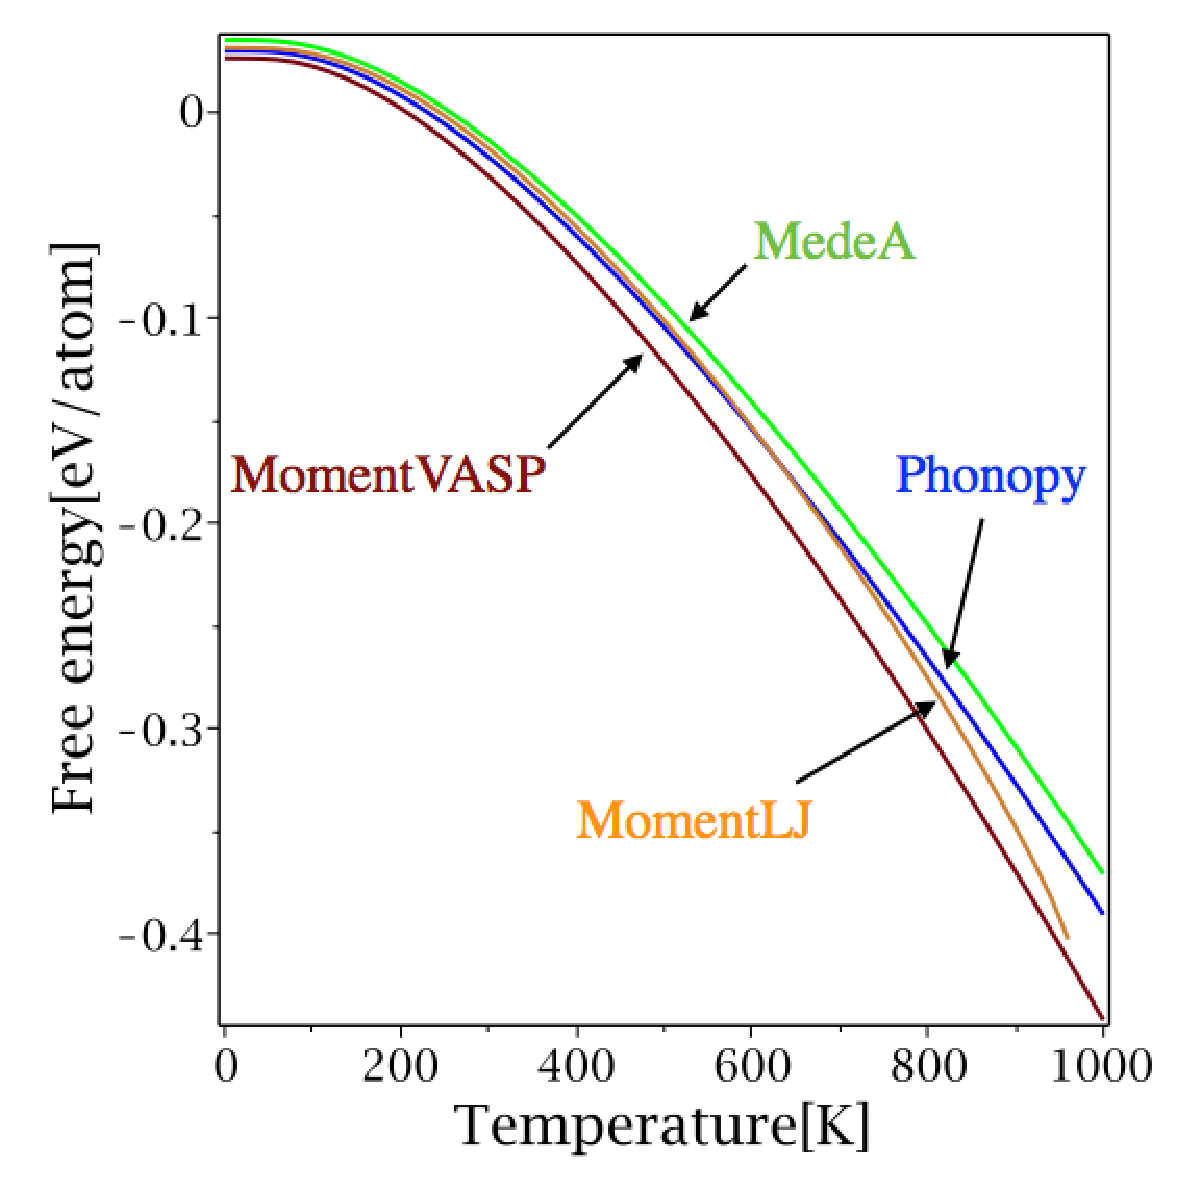
\includegraphics[keepaspectratio, scale=0.42]
  {../image_result/Cu_free_label.eps}
  \subcaption{Cu.}\label{free1}
 \end{minipage}
 \begin{minipage}[b]{0.5\linewidth}
  \centering
  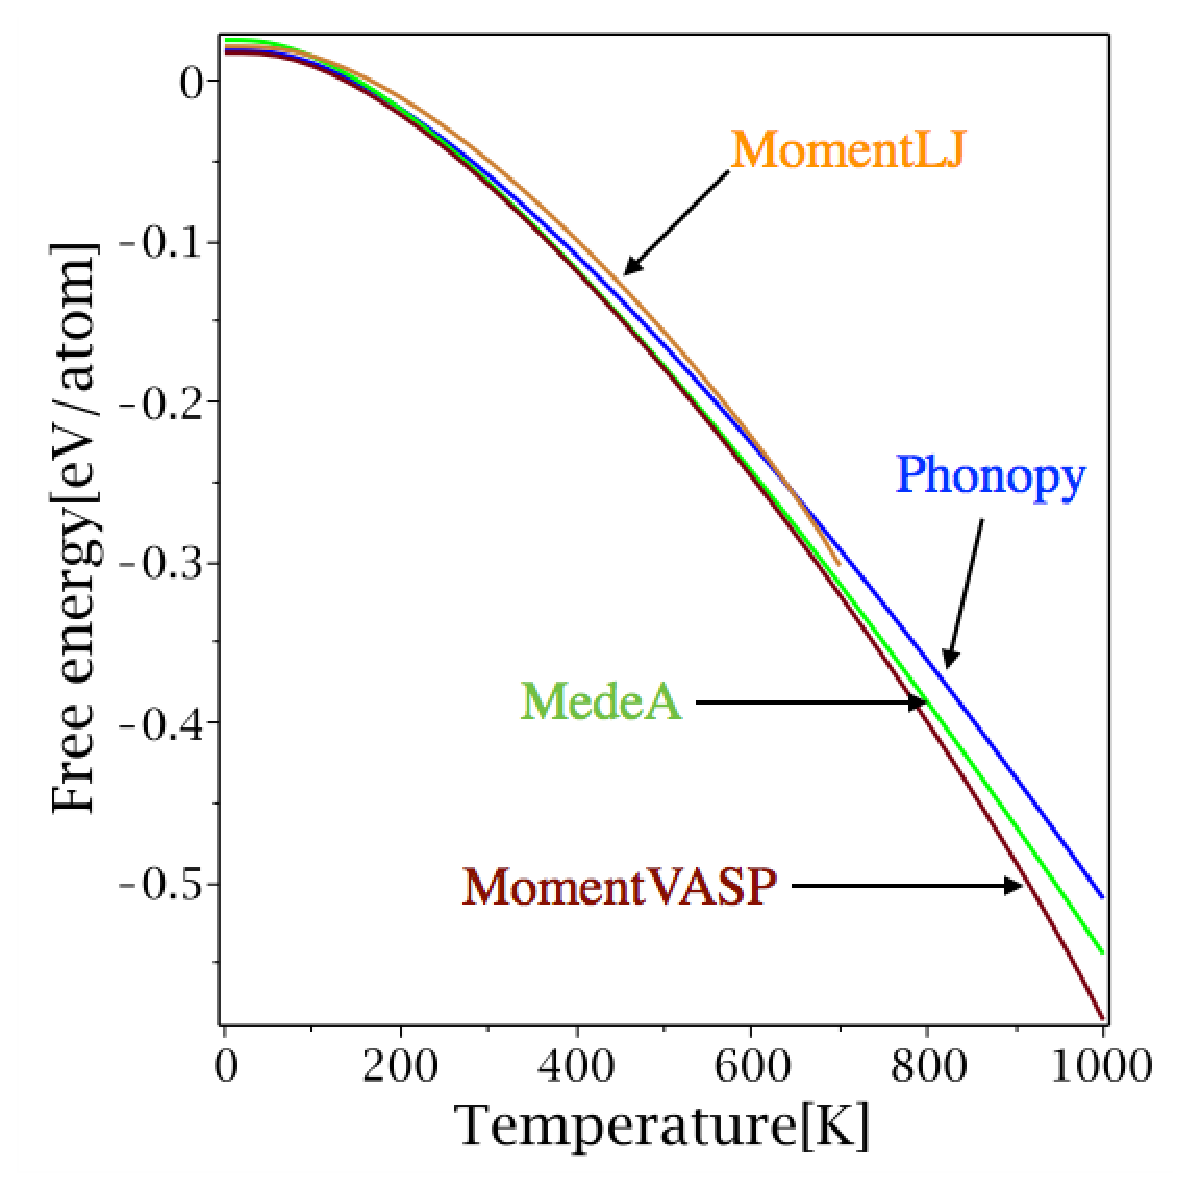
\includegraphics[keepaspectratio, scale=0.42]
  {../image_result/Ag_free_label.eps}
  \subcaption{Ag.}\label{free2}
 \end{minipage}
 \hspace{10cm}
 \begin{minipage}[b]{0.5\linewidth}
  \centering
  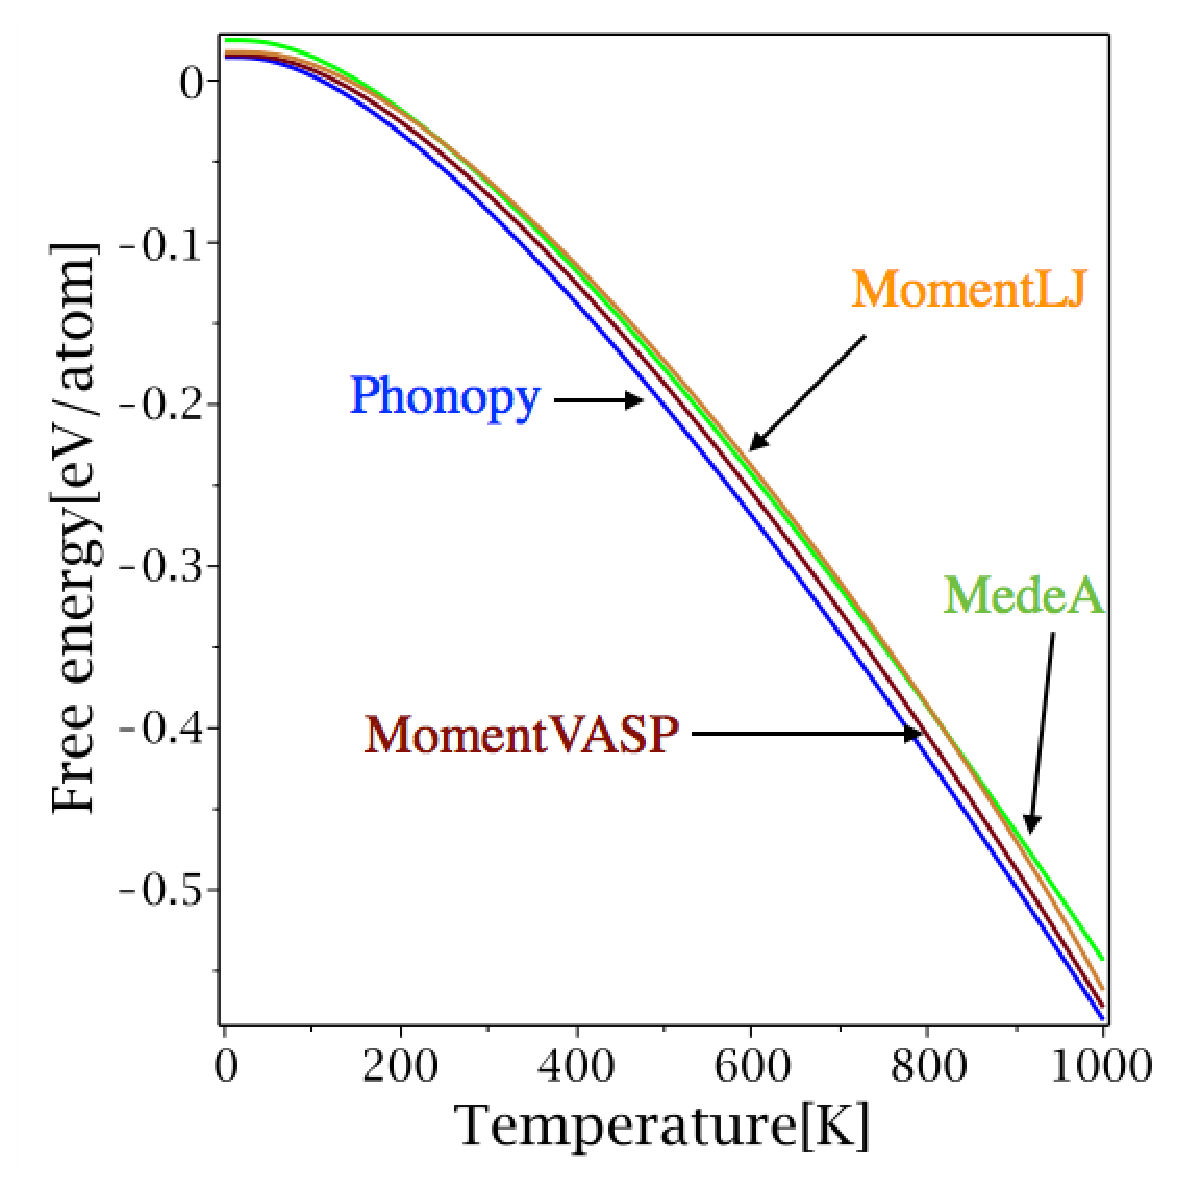
\includegraphics[keepaspectratio, scale=0.42]
  {../image_result/Au_free_label.eps}
  \subcaption{Au.}\label{free3}
 \end{minipage}
 \begin{minipage}[b]{0.5\linewidth}
  \centering
  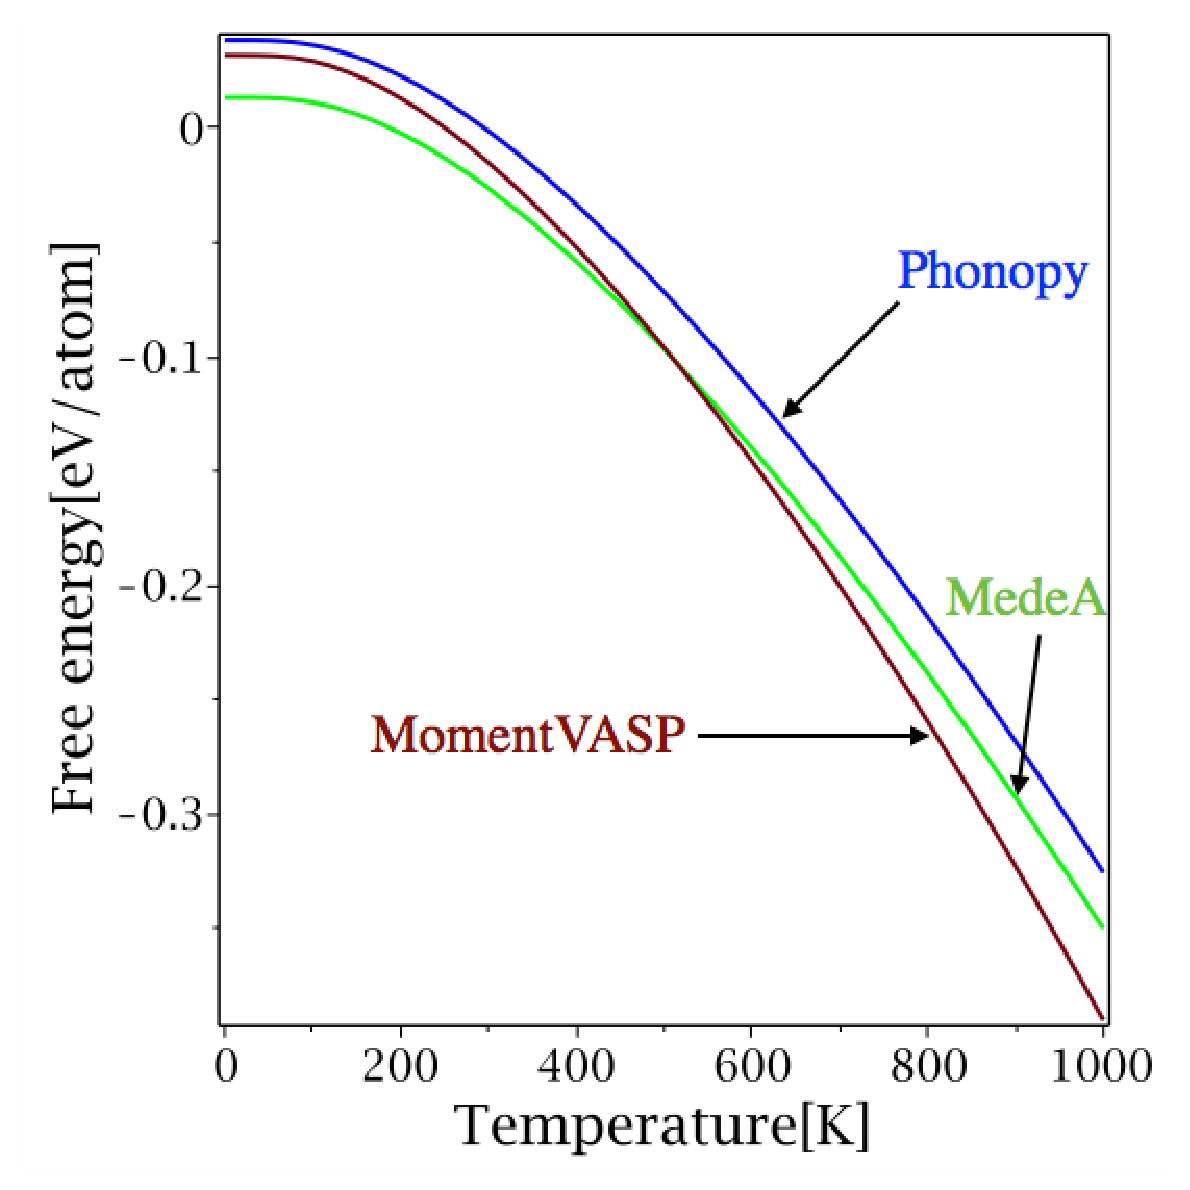
\includegraphics[keepaspectratio, scale=0.42]
  {../image_result/Al_free_label.eps}
  \subcaption{Al.}\label{free4}
 \end{minipage}
 \caption{内部エネルギー$U_0$を含まない自由エネルギーの温度依存性.MedeA, Phonopyは体積一定で計算している.}\label{fig:freeresult}
\end{figure}



\begin{table}[htbp]
  \begin{minipage}[b]{0.48\linewidth}
  \centering
  \caption{0Kと1000Kでの自由エネルギーの差(MedeA$-$MomentVASP).}
  \label{tb:free-diff}
  \begin{tabular}{ccccc}\hline
    元素 & 0K[eV] & 1000K[eV] \\ \hline \hline
    Cu & 0.008754 & 0.071124 \\
    Ag & 0.007899 & 0.041181\\
    Au & 0.009313 & 0.029068\\
    Al & -0.018484 & 0.040140\\ \hline
  \end{tabular}
 \end{minipage}
 \hspace{0.04\linewidth}
 \begin{minipage}[b]{0.48\linewidth}
 \caption{0Kと1000Kでの自由エネルギーの差(Phonopy$-$MomentVASP).}
 \label{tb:free-diff2}
  \centering
  \begin{tabular}{ccccc}\hline
    元素 & 0K[eV] & 1000K[eV] \\ \hline \hline
    Cu & 0.003605 & 0.051364  \\
    Ag & 0.001572 & 0.075705 \\
    Au & -0.001176 & -0.007870 \\
    Al & 0.006579 & 0.064626 \\ \hline
  \end{tabular}
 \end{minipage}
\end{table}




\section{内部エネルギー$U_0$を含んだ自由エネルギー}
次にPhonopyによる内部エネルギー$U_0$と熱膨張を考慮に入れた自由エネルギーとMoment法の比較を\ref{fig:freeresult2}に示す.この結果の0K,1000KでのPhonopyとMomentVASPとの自由エネルギーの差を表\ref{tb:free-diff3}に示す.
先ほどの図\ref{fig:freeresult}の結果と比べると,内部エネルギーと熱膨張を考慮に入れたことによってPhonopyの傾きがMomentVASPに近づいている.また,表\ref{tb:free-diff2}と\ref{tb:free-diff3}の自由エネルギーの差を見比べると4元素全ての値の差が小さくなっている.
特にCu, AgはAu, Alと比較すると値がよく一致している.これは図\ref{fig:heatexpantion}のCu, Agの熱膨張の結果がAu, Alよりも近い数字を出しているからだと考えられる.
この結果はMoment法は熱膨張の効果を取り入れた自由エネルギーの計算をPhonopyと同等程度に行えていることを示唆している.

\begin{figure}[htbp]
 \begin{minipage}[b]{0.5\linewidth}
  \centering
  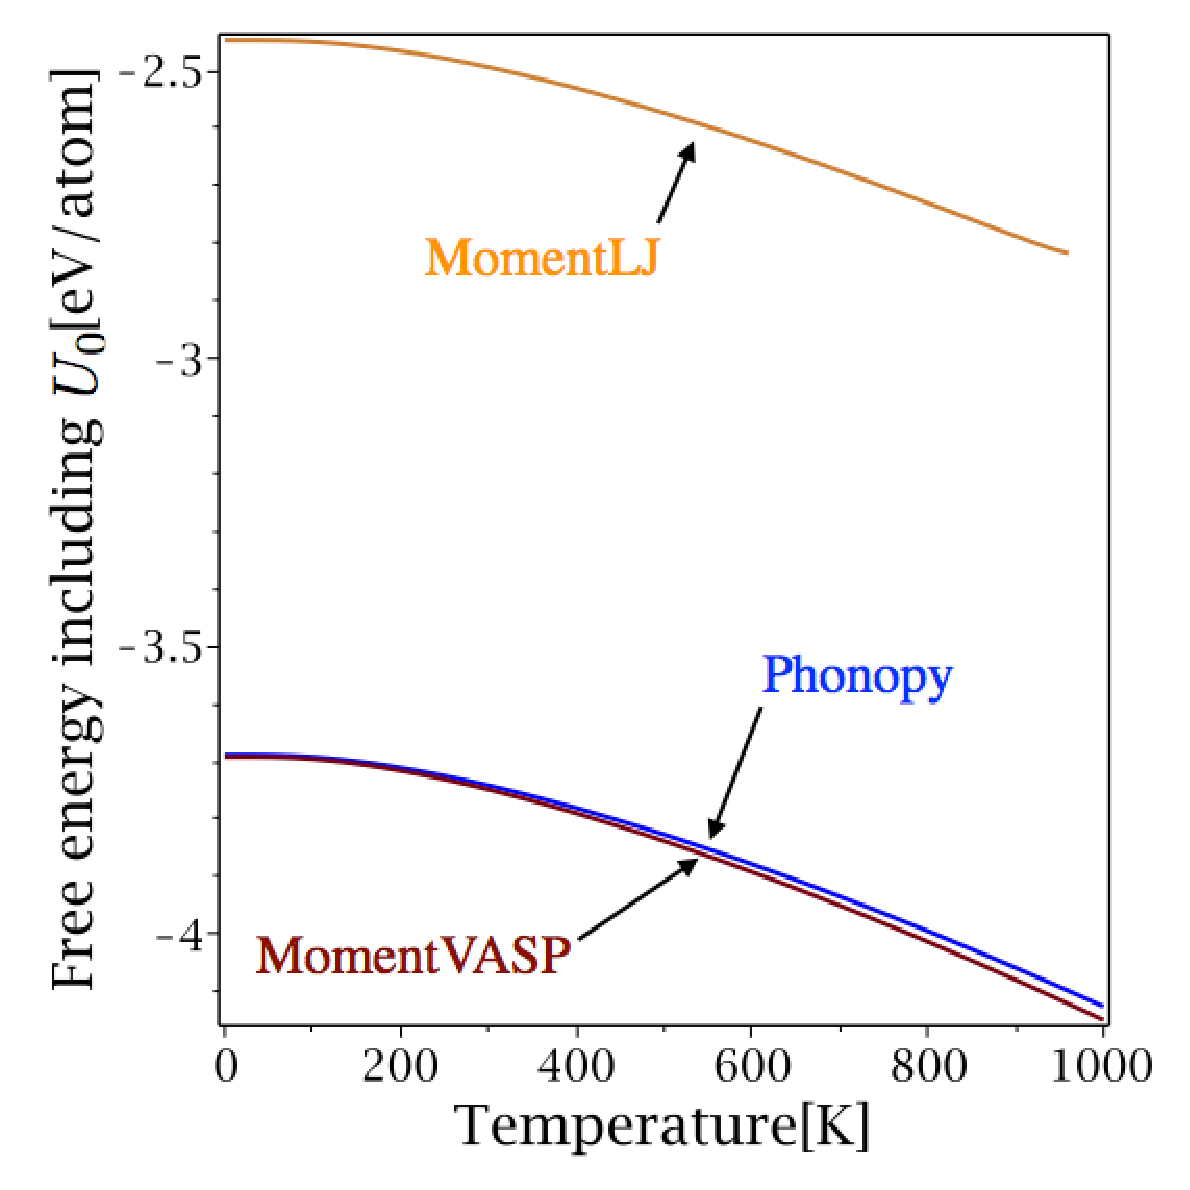
\includegraphics[keepaspectratio, scale=0.42]
  {../image_result/Cu_free_u0_label.eps}
  \subcaption{Cu.}\label{free5}
 \end{minipage}
 \begin{minipage}[b]{0.5\linewidth}
  \centering
  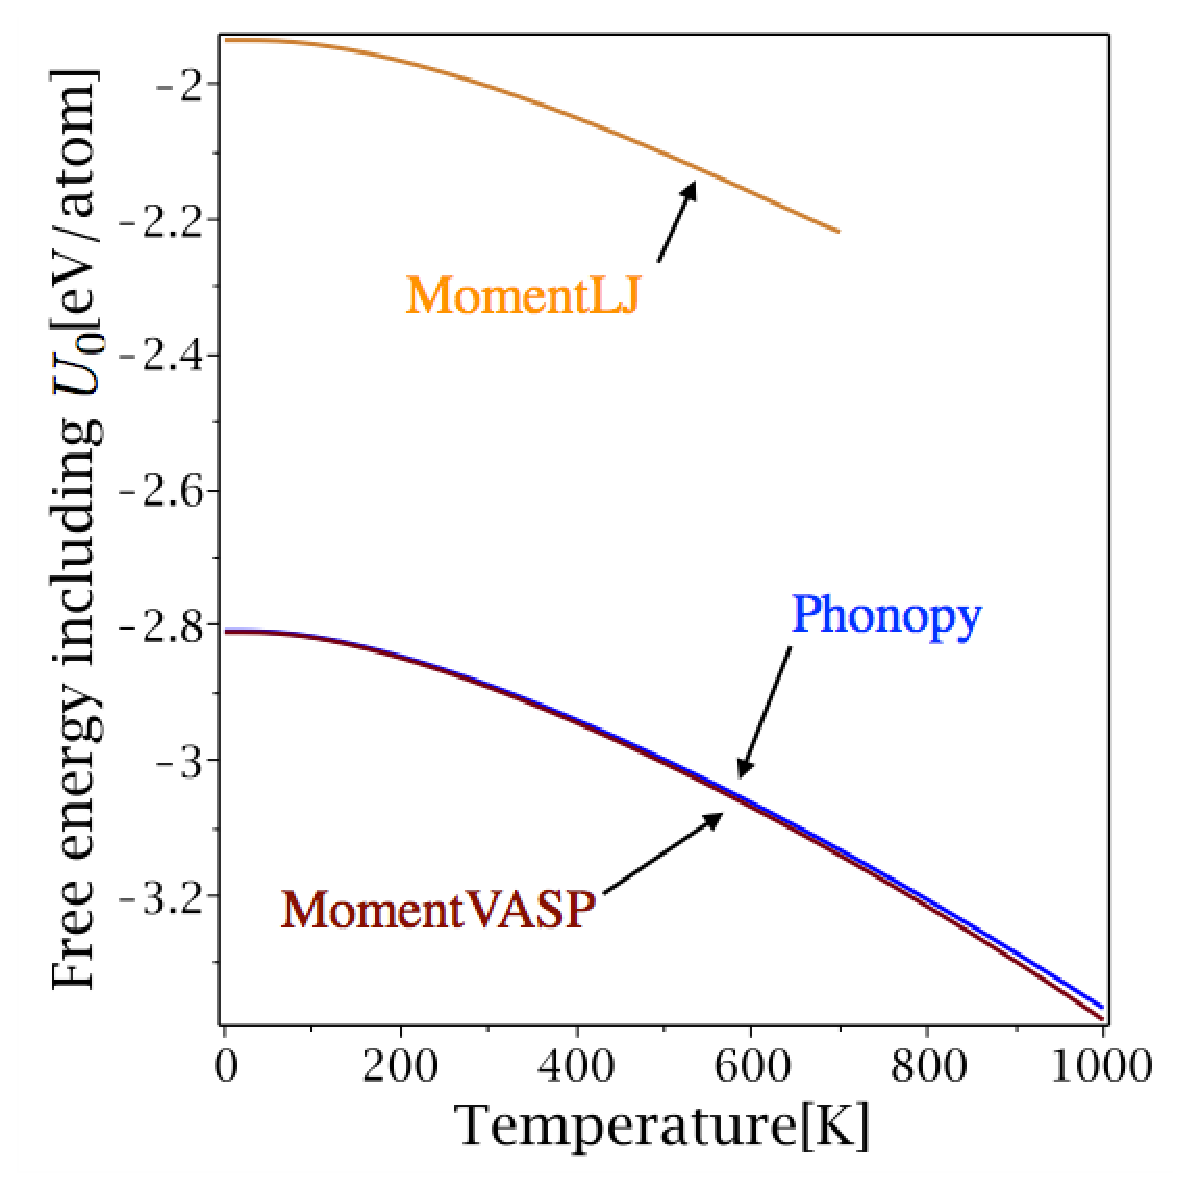
\includegraphics[keepaspectratio, scale=0.42]
  {../image_result/Ag_free_u0_label.eps}
  \subcaption{Ag.}\label{free6}
 \end{minipage}
 \hspace{10cm}
 \begin{minipage}[b]{0.5\linewidth}
  \centering
  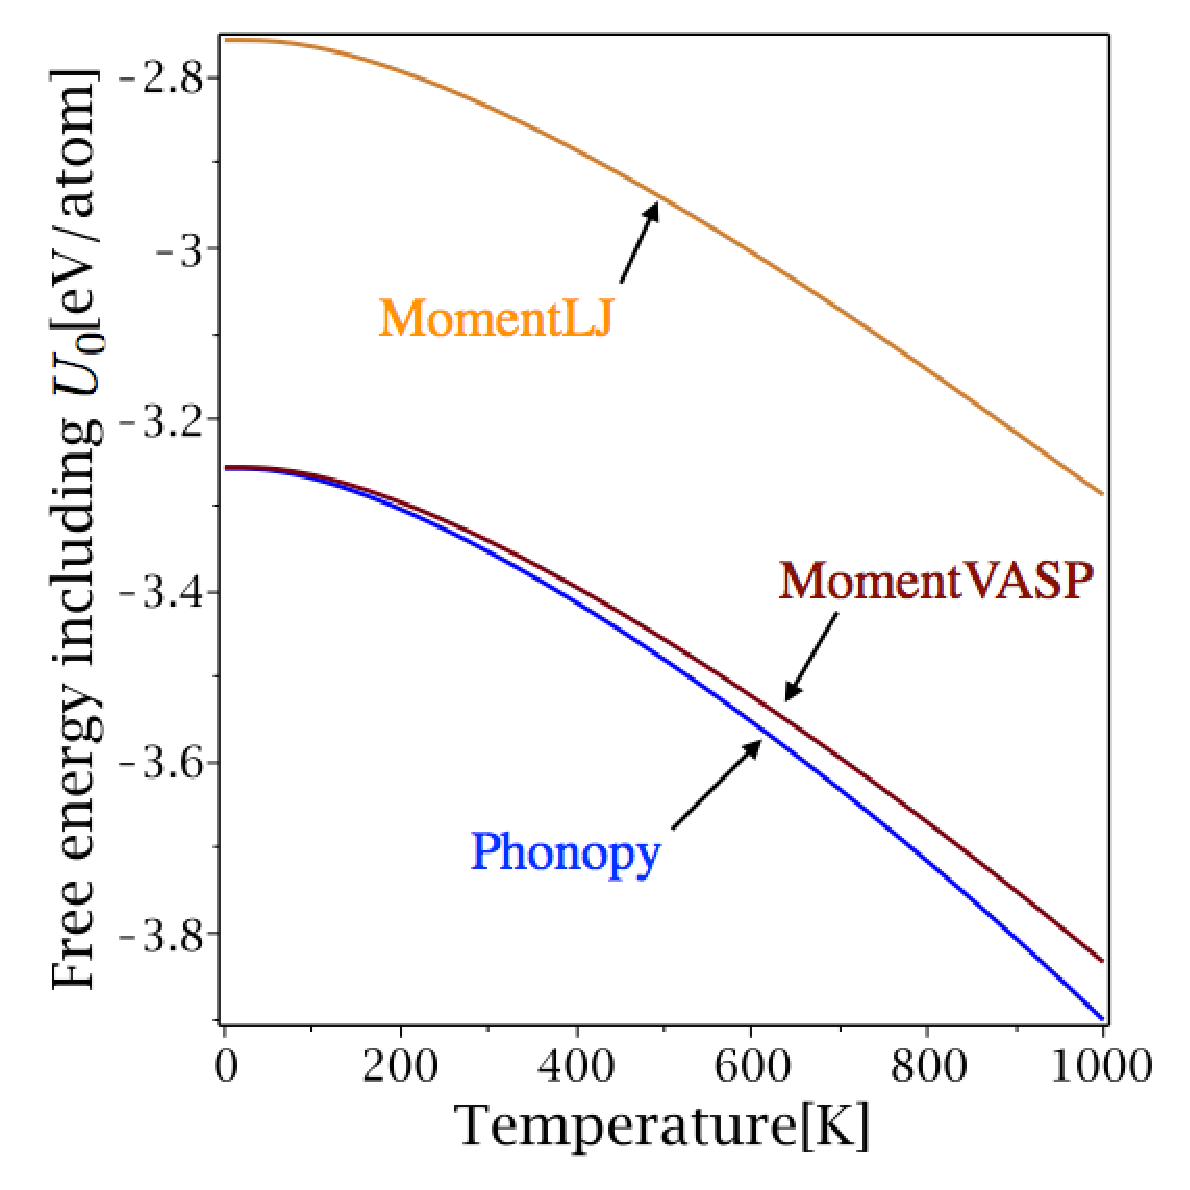
\includegraphics[keepaspectratio, scale=0.42]
  {../image_result/Au_free_u0_label.eps}
  \subcaption{Au.}\label{free7}
 \end{minipage}
 \begin{minipage}[b]{0.5\linewidth}
  \centering
  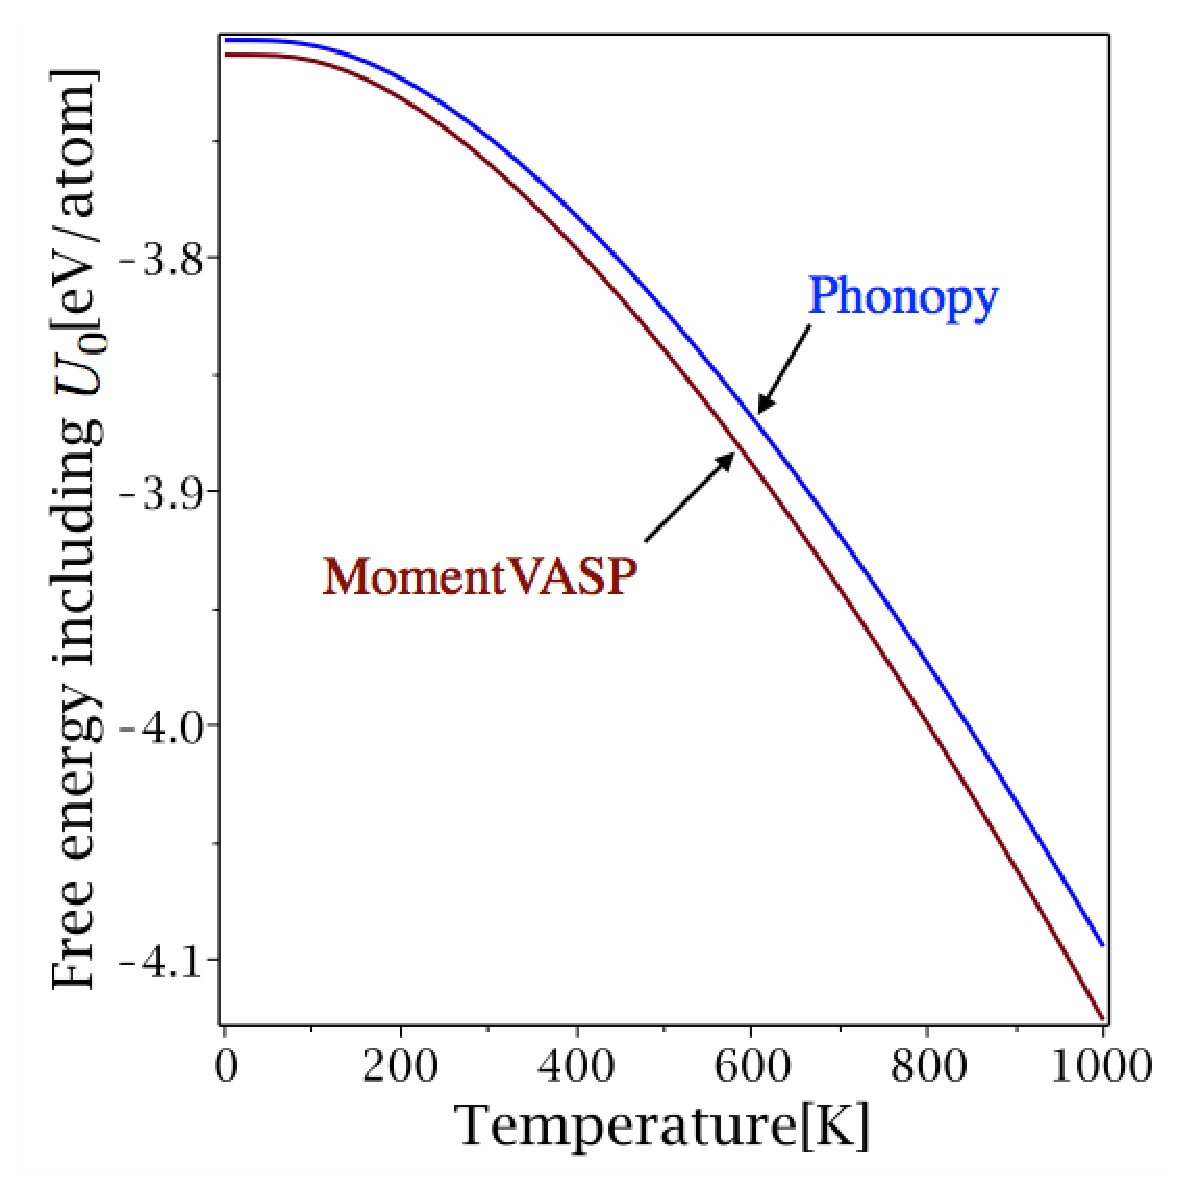
\includegraphics[keepaspectratio, scale=0.42]
  {../image_result/Al_free_u0_label.eps}
  \subcaption{Al.}\label{free8}
 \end{minipage}
 \caption{内部エネルギー$U_0$を含んだ自由エネルギーの温度依存性.Phonopyは$U_0$と熱膨張を考慮に入れて計算している.}\label{fig:freeresult2}
\end{figure}

\begin{table}[htbp]
\caption{0Kと1000Kでの$U_0$を考慮に入れた自由エネルギーの差(Phonopy$-$MomentVASP)}
  \label{tb:free-diff3}
  \centering
  \begin{tabular}{ccccc}\hline
    元素 & 0K[eV] & 1000K[eV] \\ \hline \hline
    Cu & 0.003348 & 0.023715 \\
    Ag & 0.001408 & 0.017776 \\
    Au & -0.00124 & -0.06791 \\
    Al & 0.006197 & 0.031391 \\ \hline
  \end{tabular}
\end{table}
